\subsection{Verilog}
Operator Precedence:
The order of the table tells what operation is made first, the first ones has the highest priority. The () can be used to override default. 
\subsubsection{Features of Verilog}
\begin{itemize}
	\item Case sensitive
	\item All keywords are lowercase
	\item Semicolon is the statement terminator
	\item //: single line comment
	\item /* */: multiline comment
\end{itemize} 


\subsubsection{Verilog Code structure}
Sample code to explain verilog code structure:
    \begin{lstlisting}[style={verilog-style}]
        // timescale directive tells the simulator the base units and precision of the simulation 
        `timescale 1 ns / 10 ps 
        module name (input and outputs); 
        // parameter declarations 
        parameter parameter_name = parameter value; 
        // Input output declarations 
        input in1; 
        input in2; // single bit inputs 
        output [msb:lsb] out; // a bus output 
        // internal signal register type declaration - register types (only assigned within always statements). reg register
        variable 1; 
        reg [msb:lsb] register variable 2; 
        // internal signal. net type declaration - (only assigned outside always statements) wire net variable 1; 
        // hierarchy - instantiating another module 
        reference name instance name ( 
        .pin1 (net1), 
        .pin2 (net2), 
        . 
        .pinn (netn) 
        ); 
        // synchronous procedures 
        always @ (posedge clock) 
        begin 
        . 
        end 
        // combinatinal procedures 
        always @ (signal1 or signal2 or signal3) 
        begin 
        . 
        end 
        assign net variable = combinational logic; 
        endmodule 
    \end{lstlisting}
  
Types of elements in Verilog are Wires and Registers.
\begin{itemize}
	\item \textbf{Wires} make connections between elements. They implement nets. Otherwise known as nodes in the circuit. Since wires are simply nets. They are driven by signals. They may not always have a value. So, they may have a high impedance or High-Z state. Which is neither a zero or one. But, equivalent to a floating node. 
	\item \textbf{Registers} can also make connections between elements in the code. But, registers can be a assign values. And they hold those values until the next assignment. And finally registers can drive wires. 
\end{itemize} 
	
Just a quick warning! The name register is misleading. Because Verilog registers do not necessary produce Flip flops in a FPGA or ASIC implementation. The synthesis tool will decide if the behavior really requires and actual register.


\subsubsection{Net data types}
\begin{itemize}
	\item wire: represents a node or connection
	\item tri: represents a tri-state node
	\item supply0: constant logic 0
	\item supply1: constant logic 1
\end{itemize} 

\subsubsection{Variable data types}
\begin{itemize}
	\item reg: unsigned variable of any bit size (reg signed : signed implementation)
	\item integer: signed 32-bit variable
	\item real,time,realtime: non-synthesizable
\end{itemize} 

\subsubsection{Two methods to define port connections}
\begin{itemize}
	\item By ordered list: port connections defined by the order of the port list in the lower-level module.
	\item By name: port connections defined by name, order of the port connections does not matter.
	\item Mixed is not possible.
\end{itemize} 

Parameter is value assigned to a symbolic name.
localparam is same as parameter but cannot be overwritten.


\clearpage
\subsubsection{Operators}
Verilog operators operate on several data types to produce an output. Not all Verilog operators are synthesible (can produce gates). Some operators are similar to those in the C language. Remember, you are making gates, not an algorithm (in most cases).

\begin{table}[H]
\begin{center}
\begin{tabular}{@{}lll@{}}
\toprule
\textbf{Character}                 & \textbf{Operation}             & \textbf{Type of operator}  \\ \midrule
+                                  & Add                            & Arithmatic   \\
-                                  & Subtract                       & Arithmatic   \\
/                                  & Divide                         & Arithmatic   \\
*                                  & Multiply                       & Arithmatic   \\
\%                                 & Modulus                        & Arithmatic   \\
$\sim$                             & Invert                         & bitwise      \\
\&                                 & And                            & bitwise      \\
|                                  & Or                             & bitwise      \\
$\wedge$                           & Xor                            & bitwise      \\
$\wedge$$\sim$  or $\sim$$\wedge$  & Xnor                           & bitwise      \\
\&	                               & And all bits                   & reduction    \\
$\sim$ \&	                       & Nand all bits                  & reduction    \\
|                                  & Or all bits                    & reduction    \\
$\sim$ |                           & Nor all bits                   & reduction    \\
$\wedge$                           & Xor all bits                   & reduction    \\
$\wedge$  or $\sim$$\wedge$        & Xnor all bits                  & reduction    \\
>	                               & Greater than                   & Relational   \\
<	                               & Smaller than                   & Relational   \\
>=	                               & Greater than or equal          & Relational   \\
<=	                               & Smaller than or equal          & Relational   \\
==	                               & Equality                       & Relational   \\
!=	                               & Inequality                     & Relational   \\
===	                               & Case equality                  & Relational   \\
!===	                           & Case inequality                & Relational   \\
!                                  & Not true                       & Logical      \\
\&\&                               & Both expressions true          & Logical      \\
||                                 & One or both expressions true   & Logical      \\
>>                                 & Shift right                    & shift        \\
<<                                 & Shift left                     & shift        \\
?                                  & Conditions testing             & Misc         \\
\{\}                               & Concatenate                    & Misc         \\
\{\{\}\}                           & Replicate                      & Misc         \\ \bottomrule
\end{tabular}
\end{center}
\end{table}
\clearpage


Operator Precedence:
The order of the table tells what operation is made first, the first ones has the highest priority. The () can be used to override default. 
\begin{figure}[H]
	\begin{center}
		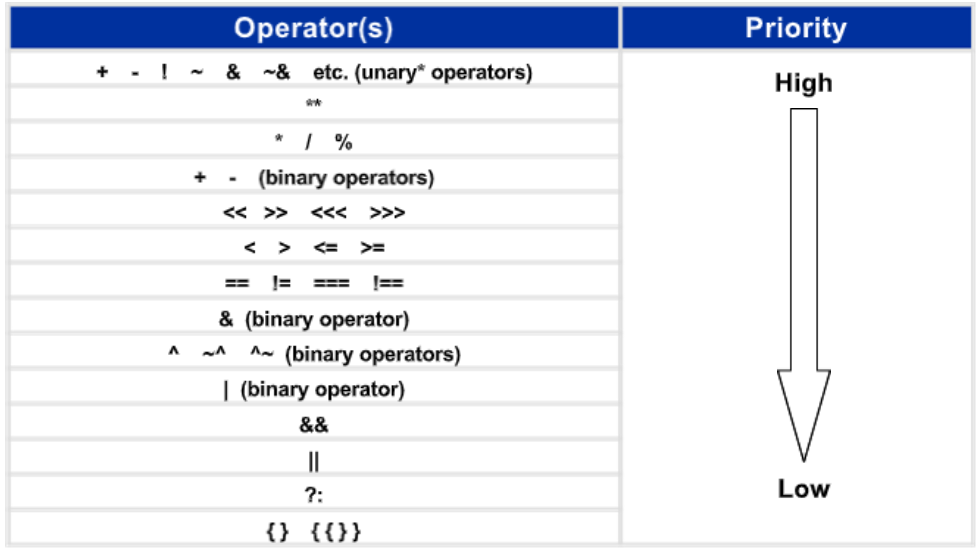
\includegraphics[width=5in]{images/OperatorPrecedence.png}
		\caption{Operator Precedence}
		\label{OperatorPrecedence}
	\end{center}
\end{figure}


\subsubsection{Assignments}
Assignment statements are categorized as follows:
\begin{description}
\item[Continuous assignments] Model the behavior of combinational logic by using expressions and operators. 
Always active: LHS is updated upon RHS changes
LHS must be a net data type.
RHS can be a bet, register or function calls.
Delay values can be assigned to model gate delays.


\item[Procedural assignments] Procedural assignments are made inside procedural blocks such as:\\
i. initial: Initializes behavioral statements for simulation. Initial block starts at 0, executes only once during simulation, and then does not execute again.\\
ii. always: Descibe the circuit functionality using behavioral statements. Block executes concurrently starting at time 0 and continuously in a looping fashion.

\par Each always and initial block represents a separate process. Processes run in parallel and start at simulation time 0. Statements inside a process execute sequentially. always and inital blocks cannot be nested.

Two types of procedural assignents:
\begin{itemize}
    \item Blocking assignments: executed in the order they are specified in a sequential block
    \item Non blocking assignments: Allow scheduling of assignments without blocking execution of  the statements that follow in a sequential block.
\end{itemize}

\end{description}

\subsubsection{RTL processes}
There are two types of RTL processes:
\begin{itemize}
    \item Combinatorial Process: sensitive to all inputs used in the combinatorial logic. ex: always @(a,b,sel)
    \item Clocked proess: sensitive to a clock or/and control signal. ex: always @(posedge clk, posedge rst)
\end{itemize}

\subsubsection{Behavioral statements}

Must be inside a procedural block (initial or always)

\begin{description}
\item[if-else] conditions are evaluated in order from top to bottom, Prioritization
\item[case] conditions are evaulated at once, No prioritization
\item[Loop] used for repetitive operations.
\begin{itemize}
    \item forever: infinite loop, non synthesizable
    \item repeat: executes a fixed number of times
    \item while: repeates until condition is achieved, non synthesizable
    \item for: executes initial assignment at the start of the loop and then executes loop body if expression is true.
\end{itemize}

\end{description}


\subsubsection{Subprograms}
Defined within a module. Uses: replacing repititive code, enhancing readability.

\begin{description}
\item[Functions] return a value based on its inputs, produces combinational logic. Always execute in zero time. Cannot pause their execution. Cannot contain delay, event, or timing control statements. Must have at least one input argument. Arguments may not be outputs, or inouts. Always return a single value. Ex: assign multOut = mult(ina, inb)

\item[Tasks] Like procedures in other languages, can be combinatorial or registered. May execute in non-zero simulation time. May contain delay, event, or timing control statements. May have zero or more input, output, or inout arguments. Ex: stmOut(nxt, first, sel, filter)

\begin{figure}[H]
	\begin{center}
		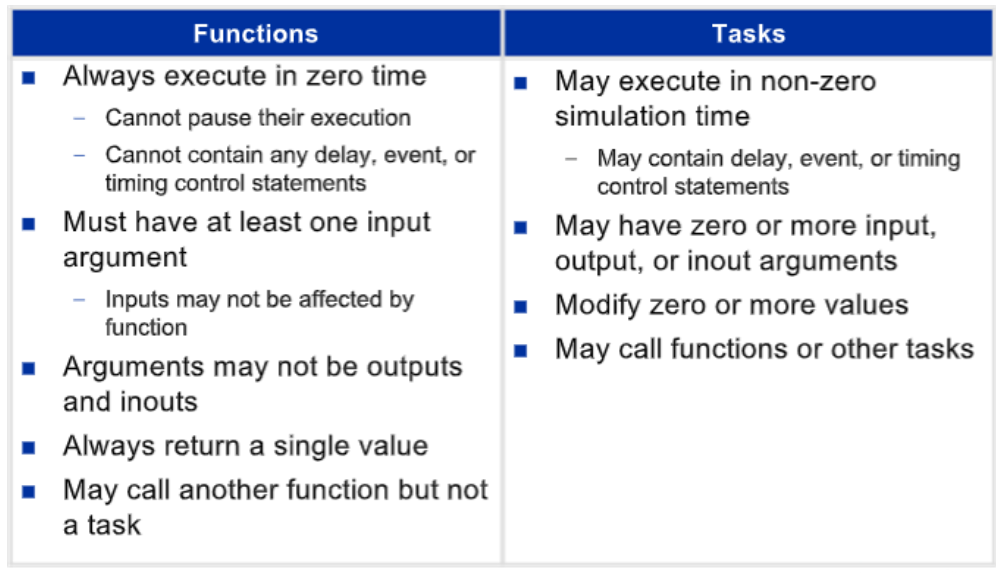
\includegraphics[width=5in]{images/VerilogFuncTasks.png}
		\caption{Verilog Functions and Tasks}
		\label{VerilogFuncTasks}
	\end{center}
\end{figure}


\end{description}
